\documentclass{article}
\usepackage[utf8]{inputenc}
\usepackage[a4paper,hmargin =1.2 in,bottom =1.2in]{geometry}
\usepackage[parfill]{parskip}
\usepackage[colorlinks = true]{hyperref}
\usepackage{fancyhdr}
\usepackage{enumitem}
\usepackage{amsmath}
\usepackage{amsthm}
\usepackage{amssymb}
\usepackage[linesnumbered,ruled,vlined]{algorithm2e}
\usepackage{listings}
\usepackage{xcolor}
\usepackage{floatrow}
\usepackage{graphicx}
\usepackage{ wasysym }
% \ bibliography style { p l a i n u r l }
% \ bibliography { b i b l i o }

\pagestyle{fancy}
\fancyhf{}
\lhead{
    200020012
}
\rhead{
    CS 747 Assignment 1
}

\cfoot{Page \thepage}
\renewcommand{\footrulewidth}{1pt}
\pagestyle{empty} 

\newtheorem{definition}{Definition}

\begin{document}
\title{CS 747 Programming Assignment 1}
\author{Adish Shah}
\date{3rd September, 2022}
\maketitle
\tableofcontents
\thispagestyle{empty}



\maketitle

\newpage
\thispagestyle{fancy}

\section{Task 1}

\subsection{UCB Algorithm}
\begin{figure}[H]
    \centerline{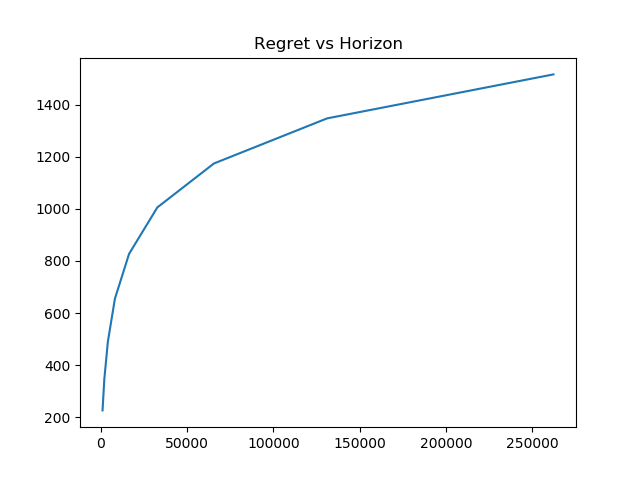
\includegraphics[scale=0.75]{task1-UCB-20220831-143044.png}}
    \caption{Regret v/s Horizon plot obtained using UCB for Task 1}
\end{figure}

The algorithm performs round-robin for the first $num\_arms$ time frames. After that 
at time t, for every arm a, we define 
\[ ucb_{a}^{t} = \hat{p}^{t}_{a} + \sqrt{\frac{2ln(t)}{u_{a}^{t}}}\]
where $\hat{p}^{t}_{a}$ is the empirical mean of rewards from arm a, and
$u_{a}^{t}$ is the number of times a has been sampled at time t. 
The arm a for which $ucb_{a}^{t}$ is maximum is pulled. This is done using the \verb!np.argmax()! function.

After receiving the reward, the corresponding empirical mean and $u_{a}^{t}$ is updated.

We can observe that the graph is increasing and concave, which is expected as the 
regret is proportional to $log(T)$, where T is the horizon.

\newpage
\thispagestyle{fancy}
\subsection{KL-UCB Algorithm}
\begin{figure}[H]
    \centerline{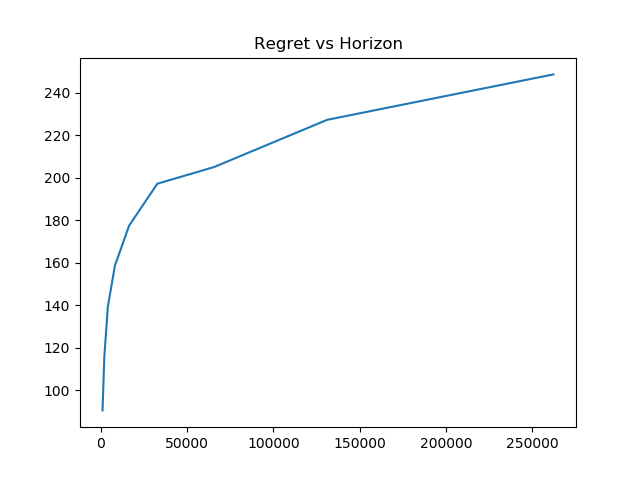
\includegraphics[scale=0.75]{task1-KL_UCB-20220831-171556.png}}
    \caption{Regret v/s Horizon plot obtained using KL-UCB for Task 1}
\end{figure}


Similar to UCB, the algorithm performs round-robin for the first $num\_arms$ time frames. 
After that at time t, for every arm a, we define 
\[ ucb-kl_{a}^{t} = max\{q \in [\hat{p}^{t}_{a},1] s.t. KL(\hat{p}^{t}_{a},q) \le \frac{ln(t) + cln(ln(t))}{u_{a}^{t}} \}\]

where $\hat{p}^{t}_{a}$ is the empirical mean of rewards from arm a, and
$u_{a}^{t}$ is the number of times a has been sampled at time t. 
 
I have chosen $c = 3$ and defined a function for $KL(p,q) = p*log(\frac{p}{q}) + (1-p)*log(\frac{1-p}{1-q})$.
The value of q is found using binary search within $10^{-4}$ of the actual value.

The arm a for which $ucb-kl_{a}^{t}$ is maximum is pulled.This is done using the \verb!np.argmax()! function.

After receiving the reward, the corresponding empirical mean and $u_{a}^{t}$ is updated.

We can observe that the graph is increasing and concave, which is expected as the 
regret is proportional to $log(T)$, where T is the horizon.
Also the regrets are lower compared to the UCB graph, which is also as expected, because
KL-UCB achieves a tighter confidence bound than UCB.

\newpage
\thispagestyle{fancy}
\subsection{Thompson Sampling}
\begin{figure}[H]
    \centerline{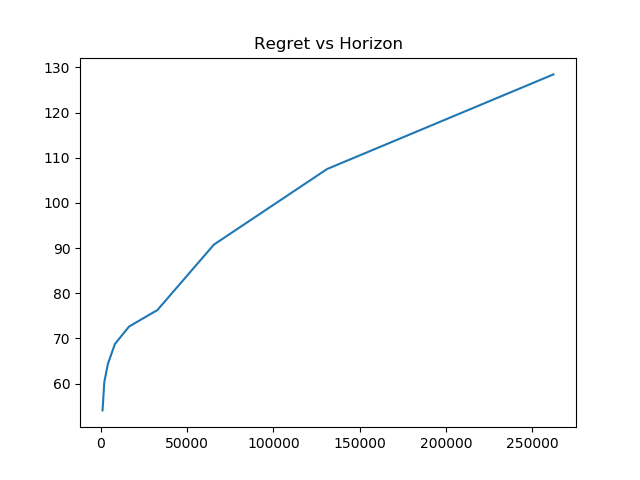
\includegraphics[scale=0.75]{task1-Thompson_Sampling-20220831-120225.png}}
    \caption{Regret v/s Horizon plot obtained using thompson sampling for Task 1}
\end{figure}


At time t, for every arm a, we have $s_{a}^{t}$ successes and $f_{a}^{t}$ failures. 
$\beta(s_{a}^{t}+1,f_{a}^{t}+1)$ represents a belief about the true mean of arm a.
So, at time t, we draw a sample from this Beta distribution for every arm a. Finally,
the one with the highest value of the sample is pulled. This is done using the \verb!np.argmax()! function.

After receiving the reward, the corresponding $s_{a}^{t}$ and $f_{a}^{t}$ are updated.

We can observe that the graph is increasing and concave, which is expected as the 
regret is proportional to $log(T)$, where T is the horizon. Overall, the regret values 
obtained from Thompson sampling are lower than UCB and KL UCB, hence we can conclude it 
performs very well practically.


\newpage
\thispagestyle{fancy}
\section{Task 2}
\begin{figure}[H]
    \centerline{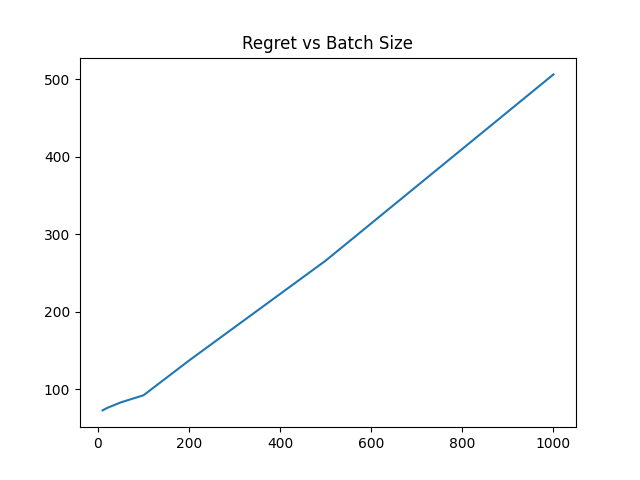
\includegraphics[scale=0.75]{task2-20220902-060224.png}}
    \caption{Regret v/s Batch Size plot obtained using batched thompson sampling for Task 2}
\end{figure}

I have implemented a \textbf{batched thompson sampling} algorithm for this task. 

The algorithm keeps track of the successes and failures of each arm.
Till batch t, we have $s_{a}^{t}$ successes and $f_{a}^{t}$ failures for arm a.  
$\beta(s_{a}^{t}+1,f_{a}^{t}+1)$ represents a belief about the true mean of arm a.
So, for every move in the new batch, we draw a sample from this Beta distribution for every arm a. The
one with the highest value of the sample is recorded and added to the list of arms to be pulled for this batch.
This gives us the set of arms to be pulled, and using the \verb!np.unique! function gives us 2 lists of
unique arms and the number of times each of them should be pulled.

After receiving the rewards, the corresponding $s_{a}^{t}$ and $f_{a}^{t}$ are updated.

We can observe that the regret linearly increases with batch size. This is because we are 
updating our belief of the true mean less frequently as bat as the batch size increases.

\newpage
\thispagestyle{fancy}
\section{Task 3}
\begin{figure}[H]
    \centerline{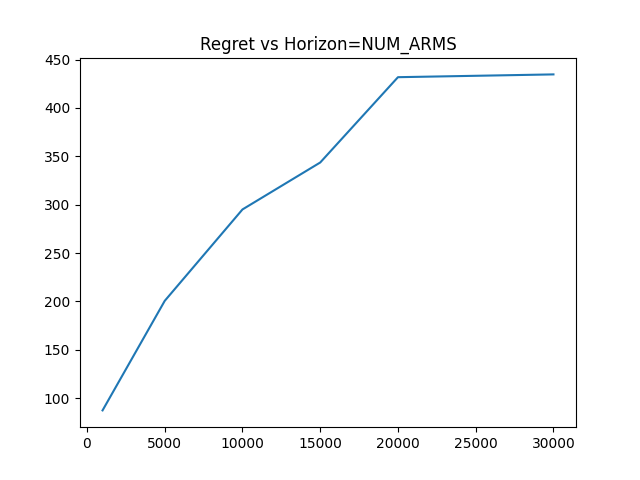
\includegraphics[scale=0.75]{task3-20220910-060229.png}}
    \caption{Regret v/s Horizon plot obtained for Task 3}
\end{figure}
In this task, since the number of arms is equal to the horizon, we cannot achieve sublinear regret, as the policies of
Infinite Exploration and Greed in the limit cannot be satisfied.

Following is my approach to the problem. A subset of the arms is chosen randomly, which contains $\mathcal{X}$ arms. Since the given bandit instance is already randomised, I simply chose the 
first $\mathcal{X}$ arms to be my subset. 
With a very high probability we get an arm that has mean more than $1 - \frac{\mathcal{X}}{N}$, where $N$ is the total number of arms.

After this, I have implemented the good old thompson sampling on this subset of arms. After experimenting a bit, I found that choosing $\mathcal{X} = \sqrt{N}$ gives low regret as compared to other values.
The graph shows an increasing trend for the most part. 
\newpage
\thispagestyle{fancy}
\section{References}
\begin{enumerate}
    \item \href{https://arxiv.org/pdf/1908.06256.pdf}{A Batched Multi-Armed Bandit Approach to News Headline Testing}
\end{enumerate}
\end{document}
